% !TeX encoding = UTF-8
% !TeX program = XeLaTeX
% !TeX spellcheck = LaTeX

\documentclass[a4paper]{article}

\usepackage{amsmath,amsfonts,amssymb}
\usepackage{mathrsfs}
\usepackage{bm}
\usepackage{extarrows}
\usepackage{geometry}
\usepackage{ntheorem}
\usepackage{hyperref}
\usepackage[ruled]{algorithm2e}
\usepackage{caption,subcaption}
\usepackage{tikz}

\usetikzlibrary{automata}

\geometry{left=2cm,right=2cm,top=2cm,bottom=2cm}

\def\UrlBreaks{\do\A\do\B\do\C\do\D\do\E\do\F\do\G\do\H\do\I\do\J\do\K\do\L\do\M\do\N\do\O\do\P\do\Q\do\R\do\S\do\T\do\U\do\V\do\W\do\X\do\Y\do\Z\do\[\do\\\do\]\do\^\do\_\do\`\do\a\do\b\do\c\do\d\do\e\do\f\do\g\do\h\do\i\do\j\do\k\do\l\do\m\do\n\do\o\do\p\do\q\do\r\do\s\do\t\do\u\do\v\do\w\do\x\do\y\do\z\do\0\do\1\do\2\do\3\do\4\do\5\do\6\do\7\do\8\do\9\do\.\do\@\do\\\do\/\do\!\do\_\do\|\do\;\do\>\do\]\do\)\do\,\do\?\do\'\do+\do\=\do\#}

\newtheorem{theorem}{Theorem}
\newtheorem{lemma}{Lemma}
\newtheorem{proposition}{Proposition}
\newtheorem{corollary}{Corollary}
\newtheorem{claim}{Claim}
\newtheorem{conjecture}{conjecture}
\newtheorem{definition}{Definition}
\newtheorem{construction}{Construction}
\newtheorem*{proof}{Proof}
\newtheorem*{answer}{Answer}
\newtheorem*{example}{Example}
\newtheorem*{counterexample}{Counterexample}

\newenvironment{exercise}[1]{
	\par
	\noindent\textbf{Exercise #1.}\quad
}{
	\par
	\bigskip
}
\newenvironment{problem}[1]{
	\par
	\noindent\textbf{Problem #1.}\quad
}{
	\par
	\bigskip
}

\DeclareMathAccent{\widehat}{\mathord}{largesymbols}{"62}
\DeclareMathOperator*{\argmax}{\arg\,\max}
\DeclareMathOperator*{\argmin}{\arg\,\min}
\DeclareMathOperator{\E}{\mathbb E}
\DeclareMathOperator{\Var}{\mathrm{Var}}
\DeclareMathOperator{\tr}{\mathrm{tr}}
\DeclareMathOperator{\poly}{\mathrm{poly}}
\newcommand{\abs}[1]{\left| #1 \right|}
\newcommand{\vabs}[1]{\left\| #1 \right\|}
\newcommand{\abra}[1]{\left\langle #1 \right\rangle}
\newcommand{\pbra}[1]{\left( #1 \right)}
\newcommand{\cbra}[1]{\left\{ #1 \right\}}
\newcommand{\sbra}[1]{\left[ #1 \right]}
\newcommand{\floorbra}[1]{\left\lfloor #1 \right\rfloor}
\newcommand{\ceilbra}[1]{\left\lceil #1 \right\rceil}
\newcommand{\bin}{\{0,1\}}
\newcommand{\ZPP}{\mathtt{ZPP}}
\newcommand{\RP}{\mathtt{RP}}
\newcommand{\coRP}{\mathtt{co}\text{-}\mathtt{RP}}
\newcommand{\per}{\text{per}}
\newcommand{\sgn}{\text{sgn}}
\newcommand{\Fbb}{\mathbb{F}}
\newcommand{\Nbb}{\mathbb{N}}
\newcommand{\Rbb}{\mathbb{R}}
\newcommand{\Zbb}{\mathbb{Z}}
\newcommand{\Sset}{\mathbb{S}}
\newcommand{\Fset}{\mathbb{F}}
\newcommand{\Nset}{\mathbb{N}}
\newcommand{\Zset}{\mathbb{Z}}
\newcommand{\Uset}{\mathbb{U}}
\newcommand{\Acal}{\mathcal{A}}
\newcommand{\Bcal}{\mathcal{B}}
\newcommand{\Ccal}{\mathcal{C}}
\newcommand{\Fcal}{\mathcal{F}}
\newcommand{\Gcal}{\mathcal{G}}
\newcommand{\qd}[2]{{\left(\frac{#1}{#2}\right)}}
\newcommand{\dv}{\ |\ }
\newcommand{\mylm}{\xLongrightarrow[lm]{}}
\newcommand{\myrm}{\xLongrightarrow[rm]{}}

\bibliographystyle{plainnat}

\title{Exercise Set --- Chapter $6$}
\date{}

\begin{document}

\maketitle

\begin{exercise}{6.2.2}\hspace{0pt}\\
\textbf{a)}
    \begin{center}
    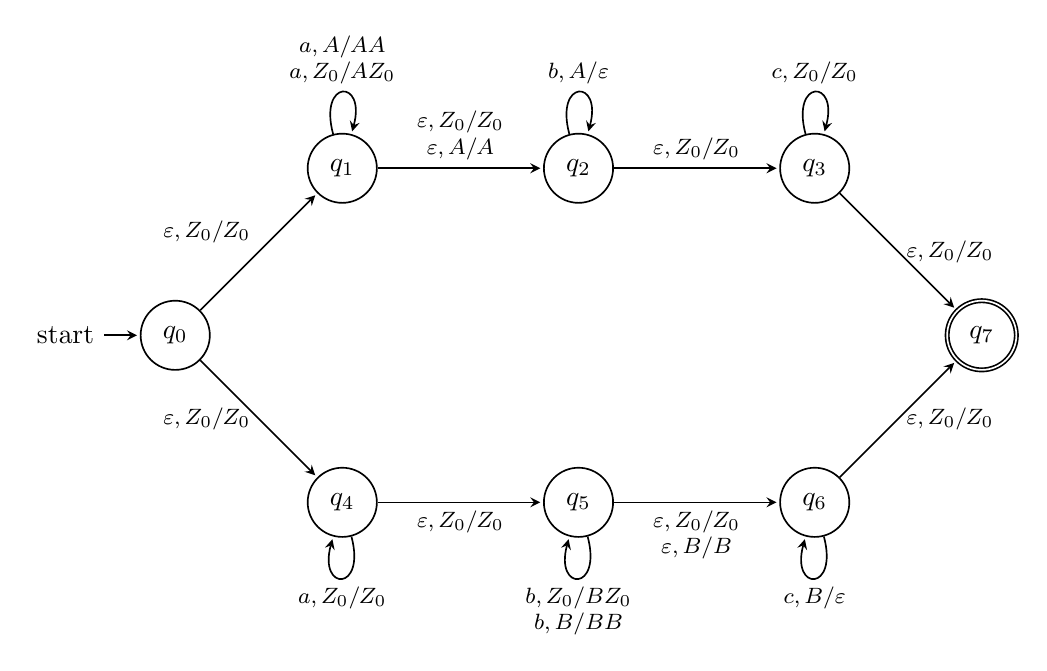
\begin{tikzpicture}[shorten >=1pt,->,>=stealth,semithick,node distance=3cm,auto,align=center]
        \node[state,initial] (q0) {$q_0$};
        \node[state] (q1) [above right of=q0] {$q_1$};
        \node[state] (q2) [right of=q1] {$q_2$};
        \node[state] (q3) [right of=q2] {$q_3$};
        \node[state] (q4) [below right of=q0] {$q_4$};
        \node[state] (q5) [right of=q4] {$q_5$};
        \node[state] (q6) [right of=q5] {$q_6$};
        \node[state,accepting] (q7) [above right of=q6] {$q_7$};

        \footnotesize
        \path[->] (q0) edge node {$\varepsilon,Z_0/Z_0$} (q1)
                       edge node[left] {$\varepsilon,Z_0/Z_0$} (q4)
                  (q1) edge[loop above] node {$a,A/AA$\\$a,Z_0/AZ_0$} ()
                       edge node {$\varepsilon,Z_0/Z_0$\\$\varepsilon,A/A$} (q2)
                  (q2) edge[loop above] node {$b,A/\varepsilon$} ()
                       edge node {$\varepsilon,Z_0/Z_0$} (q3)
                  (q3) edge[loop above] node {$c,Z_0/Z_0$} ()
                       edge node[right] {$\varepsilon,Z_0/Z_0$} (q7)
                  (q4) edge[loop below] node {$a,Z_0/Z_0$} ()
                       edge node[below] {$\varepsilon,Z_0/Z_0$} (q5)
                  (q5) edge[loop below] node {$b,Z_0/BZ_0$\\$b,B/BB$} ()
                       edge node[below] {$\varepsilon,Z_0/Z_0$\\$\varepsilon,B/B$} (q6)
                  (q6) edge[loop below] node {$c,B/\varepsilon$} ()
                       edge node[right] {$\varepsilon,Z_0/Z_0$} (q7);
    \end{tikzpicture}
    \end{center}
\textbf{b)}
    \begin{center}
    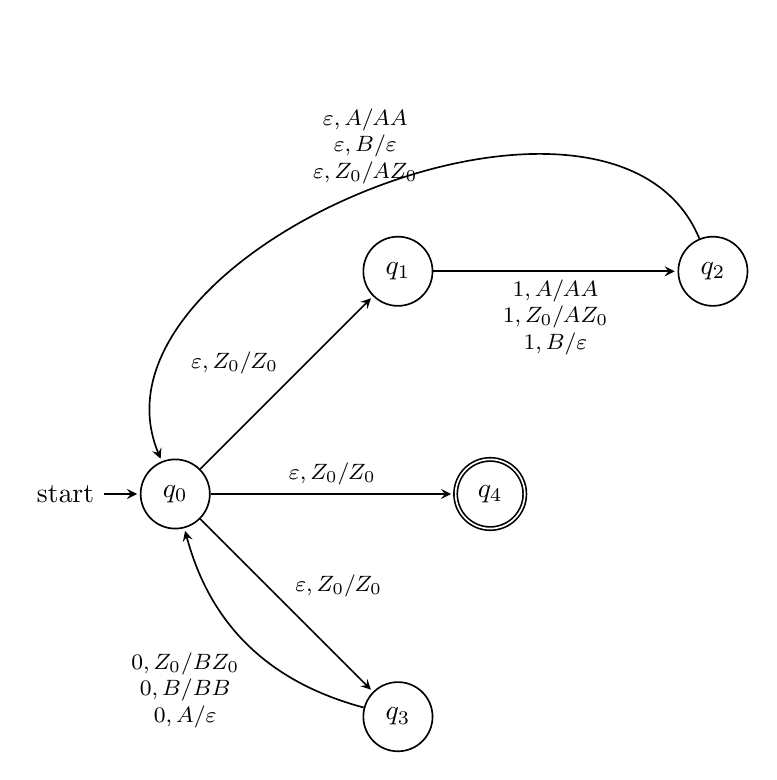
\begin{tikzpicture}[shorten >=1pt,->,>=stealth,semithick,node distance=4cm,auto,align=center]
        \node[state,initial] (q0) {$q_0$};
        \node[state] (q1) [above right of=q0] {$q_1$};
        \node[state] (q2) [right of=q1] {$q_2$};
        \node[state] (q3) [below right of=q0] {$q_3$};
        \node[state,accepting] (q4) [right of=q0] {$q_4$};

        \footnotesize
        \path[->] (q0) edge node {$\varepsilon,Z_0/Z_0$} (q4)
                       edge node {$\varepsilon,Z_0/Z_0$} (q1)
                       edge node {$\varepsilon,Z_0/Z_0$} (q3)
                  (q1) edge node[below] {$1,A/AA$\\$1,Z_0/AZ_0$\\$1,B/\varepsilon$} (q2)
                  (q2) edge[bend right=90] node[above]
                            {$\varepsilon,A/AA$\\$\varepsilon,B/\varepsilon$\\$\varepsilon,Z_0/AZ_0$} (q0)
                  (q3) edge[bend left] node {$0,Z_0/BZ_0$\\$0,B/BB$\\$0,A/\varepsilon$} (q0);
    \end{tikzpicture}
    \end{center}
\end{exercise}

\begin{exercise}{6.2.3}\hspace{0pt}\\
\textbf{a)}
    \begin{center}
    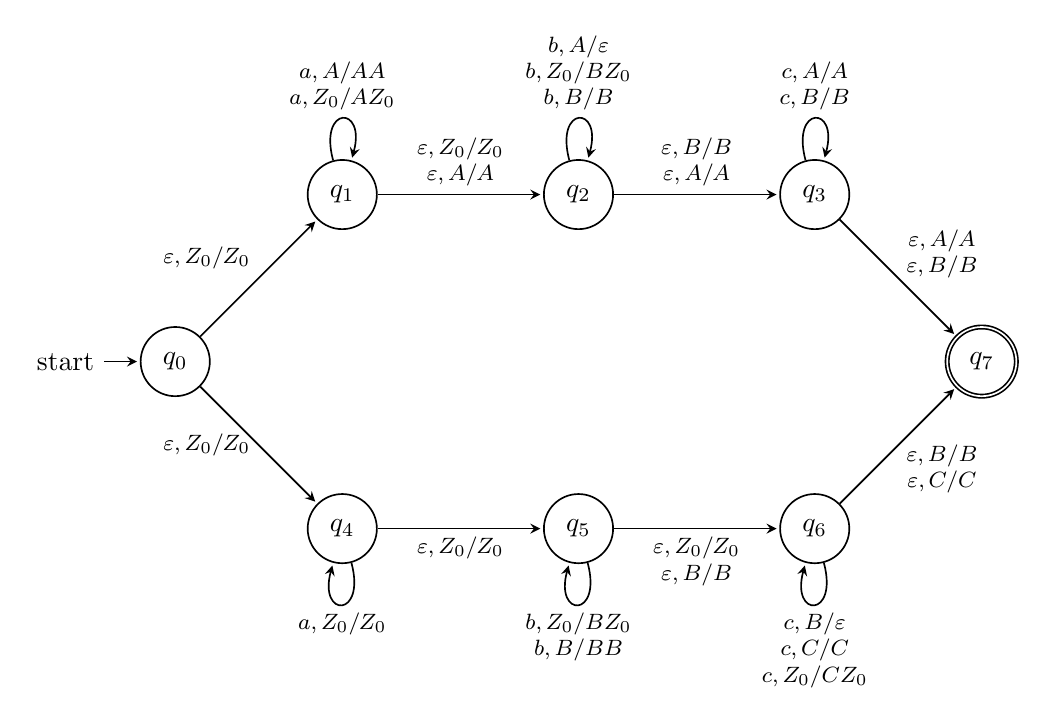
\begin{tikzpicture}[shorten >=1pt,->,>=stealth,semithick,node distance=3cm,auto,align=center]
        \node[state,initial] (q0) {$q_0$};
        \node[state] (q1) [above right of=q0] {$q_1$};
        \node[state] (q2) [right of=q1] {$q_2$};
        \node[state] (q3) [right of=q2] {$q_3$};
        \node[state] (q4) [below right of=q0] {$q_4$};
        \node[state] (q5) [right of=q4] {$q_5$};
        \node[state] (q6) [right of=q5] {$q_6$};
        \node[state,accepting] (q7) [above right of=q6] {$q_7$};

        \footnotesize
        \path[->] (q0) edge node {$\varepsilon,Z_0/Z_0$} (q1)
                       edge node[left] {$\varepsilon,Z_0/Z_0$} (q4)
                  (q1) edge[loop above] node {$a,A/AA$\\$a,Z_0/AZ_0$} ()
                       edge node {$\varepsilon,Z_0/Z_0$\\$\varepsilon,A/A$} (q2)
                  (q2) edge[loop above] node {$b,A/\varepsilon$\\$b,Z_0/BZ_0$\\$b,B/B$} ()
                       edge node {$\varepsilon,B/B$\\$\varepsilon,A/A$} (q3)
                  (q3) edge[loop above] node {$c,A/A$\\$c,B/B$} ()
                       edge node[right,yshift=3mm] {$\varepsilon,A/A$\\$\varepsilon,B/B$} (q7)
                  (q4) edge[loop below] node {$a,Z_0/Z_0$} ()
                       edge node[below] {$\varepsilon,Z_0/Z_0$} (q5)
                  (q5) edge[loop below] node {$b,Z_0/BZ_0$\\$b,B/BB$} ()
                       edge node[below] {$\varepsilon,Z_0/Z_0$\\$\varepsilon,B/B$} (q6)
                  (q6) edge[loop below] node {$c,B/\varepsilon$\\$c,C/C$\\$c,Z_0/CZ_0$} ()
                       edge node[right,yshift=-3mm] {$\varepsilon,B/B$\\$\varepsilon,C/C$} (q7);
    \end{tikzpicture}
    \end{center}
\textbf{b)} Let $\Sigma=\{a,b\}$.
    \begin{center}
    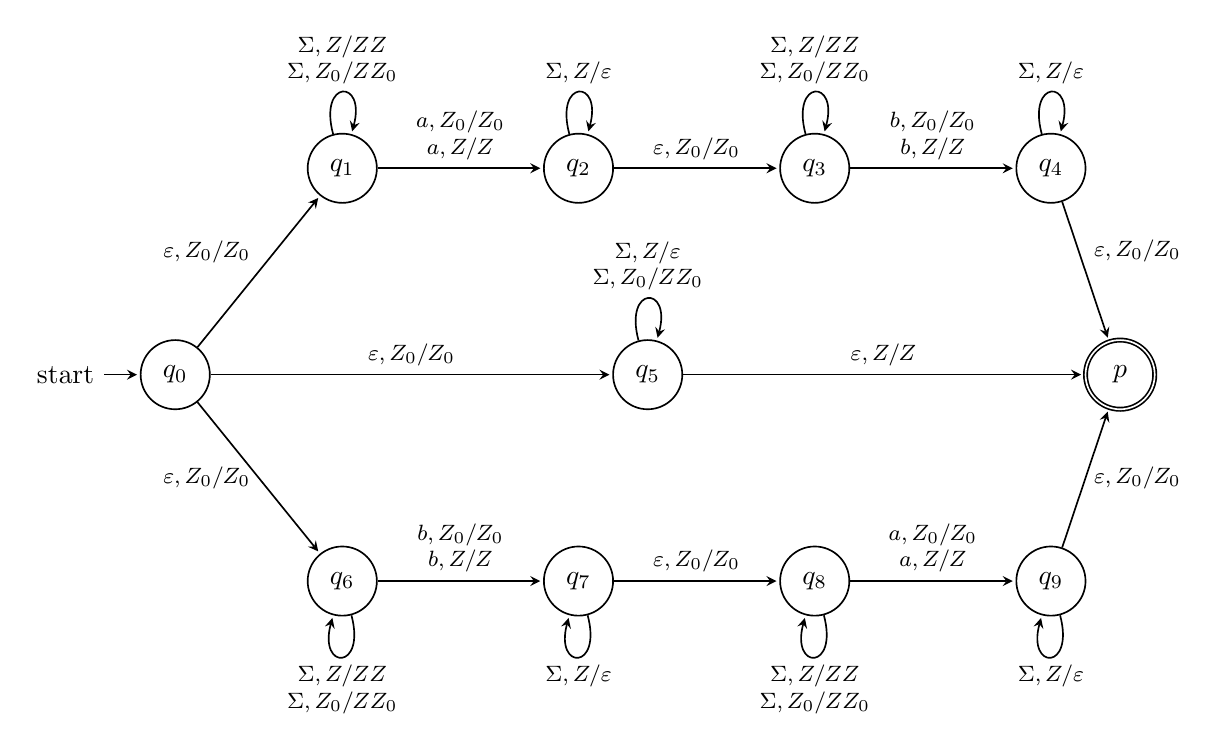
\begin{tikzpicture}[shorten >=1pt,->,>=stealth,semithick,node distance=3cm,auto,align=center]
        \node[state,initial] (q0) {$q_0$};
        \node[state] (q1) [above right of=q0,yshift=5mm] {$q_1$};
        \node[state] (q2) [right of=q1] {$q_2$};
        \node[state] (q3) [right of=q2] {$q_3$};
        \node[state] (q4) [right of=q3] {$q_4$};
        \node[state] (q5) [right of=q0,xshift=3cm] {$q_5$};
        \node[state] (q6) [below right of=q0,yshift=-5mm] {$q_6$};
        \node[state] (q7) [right of=q6] {$q_7$};
        \node[state] (q8) [right of=q7] {$q_8$};
        \node[state] (q9) [right of=q8] {$q_9$};
        \node[state,accepting] (p) [right of=q5,xshift=3cm] {$p$};

        \footnotesize
        \path[->] (q0) edge node {$\varepsilon,Z_0/Z_0$} (q1)
                       edge node {$\varepsilon,Z_0/Z_0$} (q5)
                       edge node[left] {$\varepsilon,Z_0/Z_0$} (q6)
                  (q1) edge[loop above] node {$\Sigma,Z/ZZ$\\$\Sigma,Z_0/ZZ_0$} ()
                       edge node {$a,Z_0/Z_0$\\$a,Z/Z$} (q2)
                  (q2) edge[loop above] node {$\Sigma,Z/\varepsilon$} ()
                       edge node {$\varepsilon,Z_0/Z_0$} (q3)
                  (q3) edge[loop above] node {$\Sigma,Z/ZZ$\\$\Sigma,Z_0/ZZ_0$} ()
                       edge node {$b,Z_0/Z_0$\\$b,Z/Z$} (q4)
                  (q4) edge[loop above] node {$\Sigma,Z/\varepsilon$} ()
                       edge node {$\varepsilon,Z_0/Z_0$} (p)
                  (q6) edge[loop below] node {$\Sigma,Z/ZZ$\\$\Sigma,Z_0/ZZ_0$} ()
                       edge node {$b,Z_0/Z_0$\\$b,Z/Z$} (q7)
                  (q7) edge[loop below] node {$\Sigma,Z/\varepsilon$} ()
                       edge node {$\varepsilon,Z_0/Z_0$} (q8)
                  (q8) edge[loop below] node {$\Sigma,Z/ZZ$\\$\Sigma,Z_0/ZZ_0$} ()
                       edge node {$a,Z_0/Z_0$\\$a,Z/Z$} (q9)
                  (q9) edge[loop below] node {$\Sigma,Z/\varepsilon$} ()
                       edge node[right] {$\varepsilon,Z_0/Z_0$} (p)
                  (q5) edge[loop above] node {$\Sigma,Z/\varepsilon$\\$\Sigma,Z_0/ZZ_0$} ()
                       edge node {$\varepsilon,Z/Z$} (p);
    \end{tikzpicture}
    \end{center}
\end{exercise}

\begin{exercise}{6.2.7} Assume $P=(Q,\Sigma,\Gamma,\delta,q_0,Z_0,F)$.
    In case of stack being empty, push a new stack bottom $Z_{-1}$ before $q_0$.
    \begin{center}
    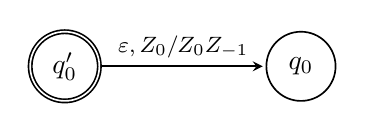
\begin{tikzpicture}[shorten >=1pt,->,>=stealth,semithick,node distance=3cm,auto,align=center]
        \node[state,accepting] (p) {$q'_0$};
        \node[state] (q) [right of=p] {$q_0$};
        \footnotesize
        \path[->] (p) edge node {$\varepsilon,Z_0/Z_0Z_{-1}$} (q);
    \end{tikzpicture}
    \end{center}
    Thus in the following proof, assume the stack will not be empty.
    \par
    Let $t=2^n\geqslant|\Gamma+1|$,
    so that characters in $\Gamma\cup\{Z_0\}$ can be uniquely encoded in binary representation of length $n$.
    Denote $\Gamma'$ be $\{b_0,b_1,\cdots,b_{t-1}\}$, where $b_i,\forall i$ is a binary string of length $n$.
    Let $\sigma:\Gamma\cup\{Z_0\}\mapsto\Gamma'$ be the bijection.\par
    Assume this is the old transition:
    \begin{center}
    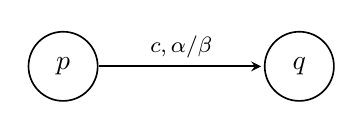
\begin{tikzpicture}[shorten >=1pt,->,>=stealth,semithick,node distance=3cm,auto,align=center]
        \node[state] (p) {$p$};
        \node[state] (q) [right of=p] {$q$};
        \footnotesize
        \path[->] (p) edge node {$c,\alpha/\beta$} (q);
    \end{tikzpicture}
    \end{center}
    Construct the new transition:
    \begin{center}
    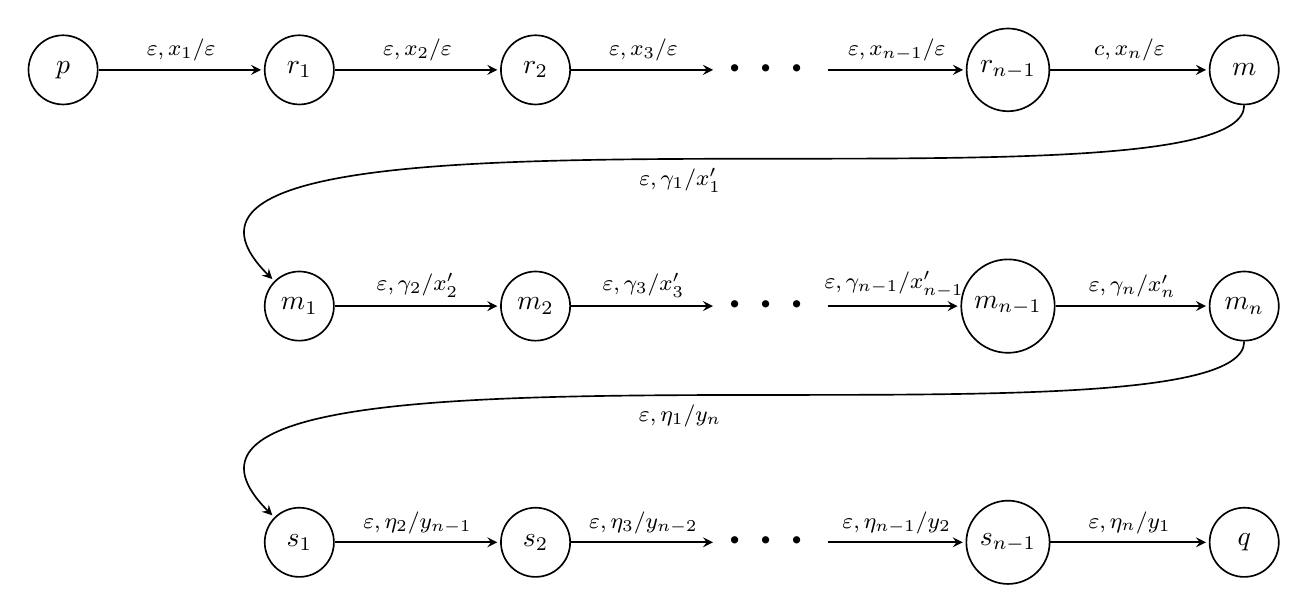
\begin{tikzpicture}[shorten >=1pt,->,>=stealth,semithick,node distance=3cm,auto,align=center]
        \node[state] (p) {$p$};
        \node[state] (r1) [right of=p] {$r_1$};
        \node[state] (r2) [right of=r1] {$r_2$};
        \node (r3) [right of=r2] {\Huge$\cdots$};
        \node[state] (r4) [right of=r3] {$r_{n-1}$};
        \node[state] (m) [right of=r4] {$m$};
        \node[state] (m1) [below of=r1] {$m_1$};
        \node[state] (m2) [right of=m1] {$m_2$};
        \node (m3) [right of=m2] {\Huge$\cdots$};
        \node[state] (m4) [right of=m3] {$m_{n-1}$};
        \node[state] (m5) [right of=m4] {$m_n$};
        \node[state] (s1) [below of=m1] {$s_1$};
        \node[state] (s2) [right of=s1] {$s_2$};
        \node (s3) [right of=s2] {\Huge$\cdots$};
        \node[state] (s4) [right of=s3] {$s_{n-1}$};
        \node[state] (s5) [right of=s4] {$q$};

        {
        \footnotesize
        \path[->] (p) edge node {$\varepsilon,x_1/\varepsilon$} (r1)
            (r1) edge node {$\varepsilon,x_2/\varepsilon$} (r2)
            (r2) edge node {$\varepsilon,x_3/\varepsilon$} (r3)
            (r3) edge node {$\varepsilon,x_{n-1}/\varepsilon$} (r4)
            (r4) edge node {$c,x_n/\varepsilon$} (m);
        \draw[->] (m) .. controls ++(0,-2) and (0,0) .. node {$\varepsilon,\gamma_1/x'_1$} (m1);
        \path[->] (m1) edge node {$\varepsilon,\gamma_2/x'_2$} (m2)
            (m2) edge node {$\varepsilon,\gamma_3/x'_3$} (m3)
            (m3) edge node {$\varepsilon,\gamma_{n-1}/x'_{n-1}$} (m4)
            (m4) edge node {$\varepsilon,\gamma_n/x'_n$} (m5);
        \draw[->] (m5) .. controls ++(0,-2) and (0,-3) .. node {$\varepsilon,\eta_1/y_n$} (s1);
        \path[->] (s1) edge node {$\varepsilon,\eta_2/y_{n-1}$} (s2)
            (s2) edge node {$\varepsilon,\eta_3/y_{n-2}$} (s3)
            (s3) edge node {$\varepsilon,\eta_{n-1}/y_2$} (s4)
            (s4) edge node {$\varepsilon,\eta_n/y_1$} (s5);
        }
    \end{tikzpicture}
    \end{center}
    where $\gamma_k,\eta_k\in\{0,1\}$ and $\overline{x_nx_{n-1}\cdots x_1}=\sigma(\alpha)$.
    $x'_k,y_k$ will be decided as follows:
    \begin{itemize}
        \item $\beta=\theta\alpha$ Then $x'_k=x_{n-k+1}\gamma_k$ and
            $y_k=z_k\eta_{n-k+1}$, where $\overline{z_nz_{n-1}\cdots z_1}=\sigma(\theta)$.
        \item $\beta=\alpha$ Then $x'_k=x_{n-k+1}\gamma_k$ and $y_k=\eta_{n-k+1}$.
        \item $\beta=\theta$ Then $x'_k=\gamma_k$ and
            $y_k=z_k\eta_{n-k+1}$, where $\overline{z_nz_{n-1}\cdots z_1}=\sigma(\theta)$.
        \item $\beta=\varepsilon$ Then $x'_k=\gamma_k$ and $y_k=\eta_{n-k+1}$.
    \end{itemize}
    The intuition is that the first line pops out the top and makes match with $c$;
    the second line pushes the old top back if necessary;
    the third line pushes the new top if necessary.\par
    Therefore, this new PDA simulates the action of $P$ and it meets the requirement.
\end{exercise}

\begin{exercise}{6.3.3} Since $P$, which is a PDA by empty stack,
has no rule for popping out $Z_0$ in stack,
$P$ actually accepts nothing. Thus the corresponding CFG is $L(G)=\varnothing$
as well.
\end{exercise}

\begin{exercise}{6.3.6}
    First convert $P$ to CFG $G$, then convert the CFG $G$ to PDA $P_1$.
    According to the construct algorithm, $P_1$ has only one state and $N(P_1)=L(G)=N(P)$.
\end{exercise}

\begin{exercise}{6.4.2}\hspace{0pt}\\
\textbf{a)}
    \begin{center}
    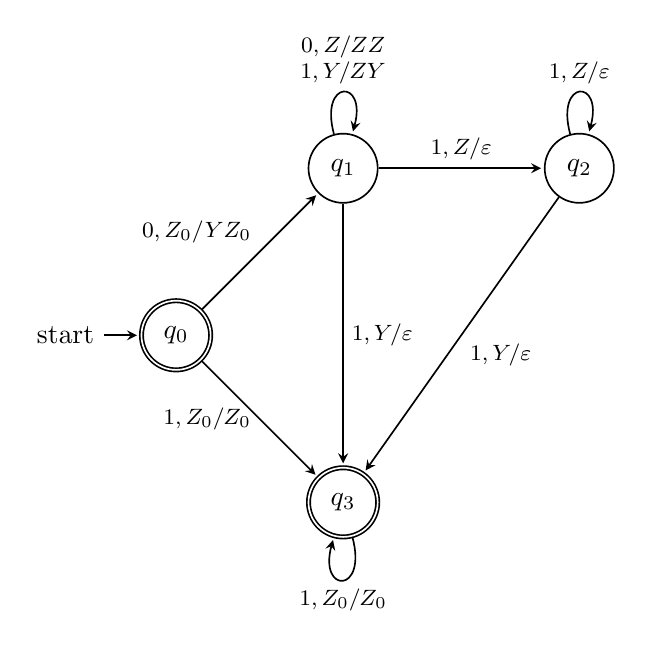
\begin{tikzpicture}[shorten >=1pt,->,>=stealth,semithick,node distance=3cm,auto,align=center]
        \node[state,initial,accepting] (q0) {$q_0$};
        \node[state] (q1) [above right of=q0] {$q_1$};
        \node[state] (q2) [right of=q1] {$q_2$};
        \node[state,accepting] (q3) [below right of=q0] {$q_3$};

        \footnotesize
        \path[->] (q0) edge node {$0,Z_0/YZ_0$} (q1)
                       edge node[left] {$1,Z_0/Z_0$} (q3)
                  (q1) edge[loop above] node {$0,Z/ZZ$\\$1,Y/ZY$} ()
                       edge node {$1,Z/\varepsilon$} (q2)
                       edge node {$1,Y/\varepsilon$} (q3)
                  (q2) edge[loop above] node {$1,Z/\varepsilon$} ()
                       edge node {$1,Y/\varepsilon$} (q3)
                  (q3) edge[loop below] node {$1,Z_0/Z_0$} ();
    \end{tikzpicture}
    \end{center}
\textbf{b)}
    \begin{center}
    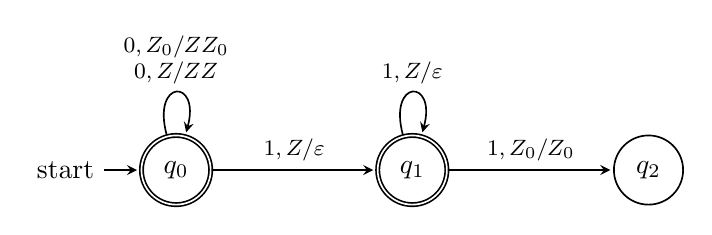
\begin{tikzpicture}[shorten >=1pt,->,>=stealth,semithick,node distance=3cm,auto,align=center]
        \node[state,initial,accepting] (q0) {$q_0$};
        \node[state,accepting] (q1) [right of=q0] {$q_1$};
        \node[state] (q2) [right of=q1] {$q_2$};

        \footnotesize
        \path[->] (q0) edge[loop above] node {$0,Z_0/ZZ_0$\\$0,Z/ZZ$} ()
                       edge node {$1,Z/\varepsilon$} (q1)
                  (q1) edge[loop above] node {$1,Z/\varepsilon$} ()
                       edge node {$1,Z_0/Z_0$} (q2);
    \end{tikzpicture}
    \end{center}
\textbf{c)}
    \begin{center}
    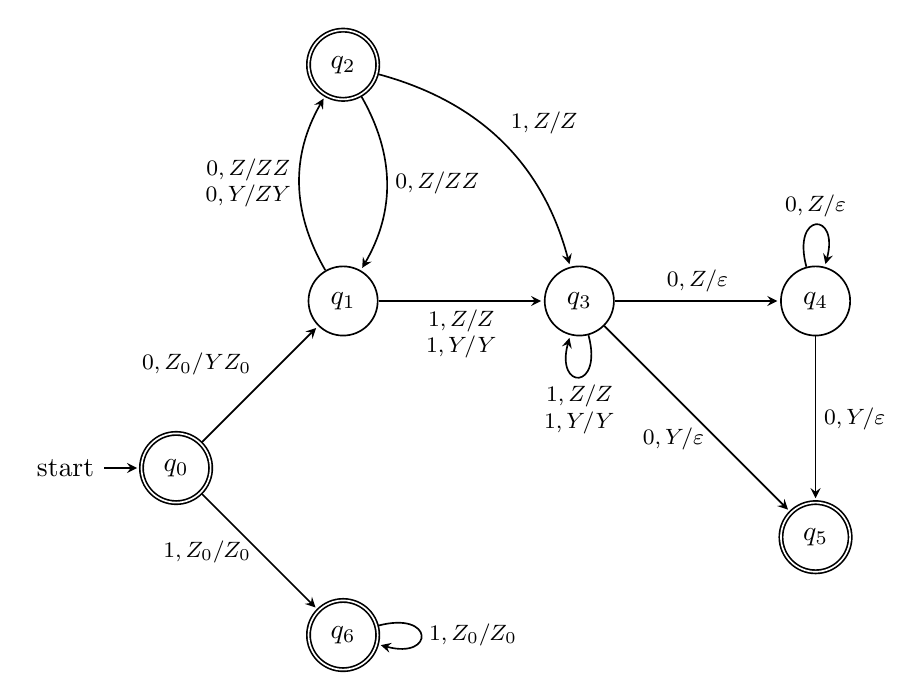
\begin{tikzpicture}[shorten >=1pt,->,>=stealth,semithick,node distance=3cm,auto,align=center]
        \node[state,initial,accepting] (q0) {$q_0$};
        \node[state] (q1) [above right of=q0] {$q_1$};
        \node[state,accepting] (q2) [above of=q1] {$q_2$};
        \node[state] (q3) [right of=q1] {$q_3$};
        \node[state] (q4) [right of=q3] {$q_4$};
        \node[state,accepting] (q5) [below of=q4] {$q_5$};
        \node[state,accepting] (q6) [below right of=q0] {$q_6$};

        \footnotesize
        \path[->] (q0) edge node {$0,Z_0/YZ_0$} (q1)
                       edge node[left] {$1,Z_0/Z_0$} (q6)
                  (q6) edge[loop right] node {$1,Z_0/Z_0$} ()
                  (q1) edge[bend left] node {$0,Z/ZZ$\\$0,Y/ZY$} (q2)
                       edge node[below] {$1,Z/Z$\\$1,Y/Y$} (q3)
                  (q2) edge[bend left] node {$0,Z/ZZ$} (q1)
                       edge[bend left] node {$1,Z/Z$} (q3)
                  (q3) edge[loop below] node {$1,Z/Z$\\$1,Y/Y$} ()
                       edge node {$0,Z/\varepsilon$} (q4)
                       edge node[below,xshift=-3mm] {$0,Y/\varepsilon$} (q5)
                  (q4) edge[loop above] node {$0,Z/\varepsilon$} ()
                       edge node {$0,Y/\varepsilon$} (q5);
    \end{tikzpicture}
    \end{center}
\end{exercise}

\end{document}
